\documentclass[11pt]{standalone}
\usepackage{amssymb}
\usepackage{amsmath}
\usepackage[no-math]{fontspec}
\usepackage{unicode-math}
\usepackage{libertinus}
\usepackage{pgf,xcolor}
\usepackage{tikz}
\usetikzlibrary{arrows.meta, backgrounds, calc}
\usepackage{pgfplots}
\pgfplotsset{compat=newest}

\definecolor{my_darkgray}{HTML}{484949}
\definecolor{my_lightgray}{HTML}{F3F4F4}
\definecolor{my_darkblue}{HTML}{005A94}
\definecolor{my_lightblue}{HTML}{CCDEE9}
\definecolor{my_yellow}{HTML}{FFEC7F}
\definecolor{my_red}{HTML}{E60000}
\definecolor{my_orange}{HTML}{E87846}

\begin{document}
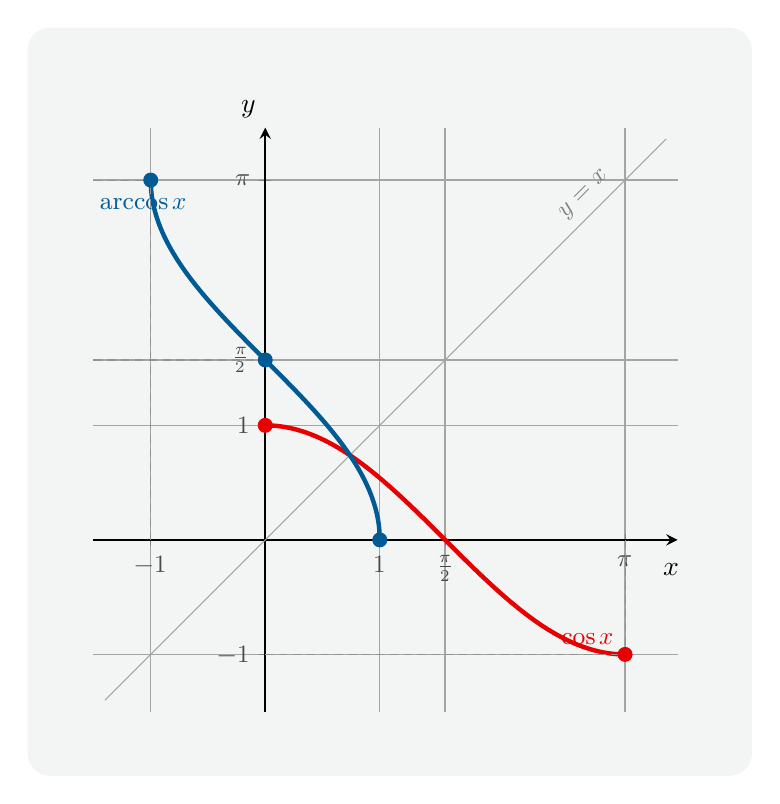
\begin{tikzpicture}[
    show background rectangle,
    background rectangle/.style={fill=my_lightgray, rounded corners=8pt},
    inner frame sep=0.8cm
]

% arccos(x): domain [-1, 1], range [0, π]
% cos restricted to [0, π]: domain [0, π], range [-1, 1]
% Both live in the window [-1, π] × [-1, π]; axis equal preserves the
% mirror symmetry across y = x.
\begin{axis}[
    axis lines = center,
    xlabel = {$x$},
    ylabel = {$y$},
    xlabel style = {at={(axis cs:3.55,0)}, anchor=north, yshift=-5pt},
    ylabel style = {anchor=south east},
    grid = both,
    grid style = {line width=0.3pt, draw=my_darkgray!30},
    major grid style = {line width=0.5pt, draw=my_darkgray!50},
    axis equal,
    axis line style = {thick},
    xmin = -1.5, xmax = 3.6,
    ymin = -1.5, ymax = 3.6,
    xtick = {-1, 0, 1, 1.5708, 3.14159},
    xticklabels = {$-1$, $0$, $1$, $\tfrac{\pi}{2}$, $\pi$},
    ytick = {-1, 0, 1, 1.5708, 3.14159},
    yticklabels = {$-1$, $0$, $1$, $\tfrac{\pi}{2}$, $\pi$},
    yticklabel style = {font=\small, text=my_darkgray},
    xticklabel style = {font=\small, text=my_darkgray},
    width=9cm, height=9cm,
    clip=false,
]

% Diagonal y = x: mirror axis for the inverse relationship
\addplot[
    draw=my_darkgray!50,
    thin,
    domain=-1.4:3.5
]{ x };
\node[anchor=south, rotate=45, font=\small, text=my_darkgray!70]
    at (axis cs:2.9, 2.9) {$y = x$};

% cos(x) restricted to [0, π]: the function being inverted
\addplot[
    draw=my_red,
    samples=400,
    ultra thick,
    domain=0:3.14159
]{ cos(deg(x)) };

% Closed endpoints of cos on [0, π]: (0, 1) and (π, -1)
\addplot[
    mark=*,
    mark size=2.5pt,
    only marks,
    draw=my_red,
    fill=my_red
] coordinates {(0, 1) (3.14159, -1)};

\node[anchor=south west, font=\small, text=my_red]
    at (axis cs:2.5, -1) {$\cos x$};

% arccos(x) on its full closed domain [-1, 1]
\addplot[
    draw=my_darkblue,
    samples=500,
    ultra thick,
    domain=-1:1
]{ acos(x) * pi / 180 };

% Closed endpoints: (-1, π) and (1, 0)
\addplot[
    mark=*,
    mark size=2.5pt,
    only marks,
    draw=my_darkblue,
    fill=my_darkblue
] coordinates {(-1, 3.14159) (1, 0)};

\node[anchor=south east, font=\small, text=my_darkblue]
    at (axis cs:-0.6, 2.8) {$\arccos x$};

% Mark (0, π/2): arccos(0) = π/2, midpoint of the range
\addplot[
    mark=*,
    mark size=2.5pt,
    only marks,
    draw=my_darkblue,
    fill=my_darkblue
] coordinates {(0, 1.5708)};

% Dashed reference lines for the endpoint (-1, π)
\addplot[draw=my_darkgray!60, densely dashed, thin]
    coordinates {(-1, 0) (-1, 3.14159)};
\addplot[draw=my_darkgray!60, densely dashed, thin]
    coordinates {(-1.5, 3.14159) (-1, 3.14159)};

% Dashed reference lines for the endpoint (π, -1) of cos
\addplot[draw=my_darkgray!60, densely dashed, thin]
    coordinates {(3.14159, 0) (3.14159, -1)};
\addplot[draw=my_darkgray!60, densely dashed, thin]
    coordinates {(0, -1) (3.14159, -1)};

% Dashed reference lines for the midpoint (0, π/2) of arccos
\addplot[draw=my_darkgray!60, densely dashed, thin]
    coordinates {(-1.5, 1.5708) (0, 1.5708)};

\end{axis}
\end{tikzpicture}
\end{document}
